\section{Exercise 1: Smart Home Alarm System (Scala - Pekko)}
L'obiettivo dell'esercizio è la progettazione e implementazione di un sistema di allarme domestico. Il sistema deve gestire segnali asincroni provenienti da una rete di sensori, e interazioni utente tramite un tastierino, reagendo in modo differente in base al proprio stato.

\subsection{Analisi del Problema}
Inizialmente sono stati analizzati gli stati e le transizioni del sistema, identificando chiaramente le fasi di \textbf{Disarmed}, \textbf{Exit Delay}, \textbf{Armed}, \textbf{Entry Delay} e \textbf{Alarm}. Ogni stato ha comportamenti specifici in risposta a eventi come l'inserimento del PIN, il rilevamento di un sensore o lo scadere di un timer.

\subsubsection{Macchina a Stati e Vincoli Temporali}
Il cuore del sistema in grado di gestire i principali stati, è il Guardian, che deve implementare una macchina a stati finiti per garantire che le transizioni avvengano in modo coerente e prevedibile. Inoltre, i vincoli temporali (Exit Delay ed Entry Delay) richiedono l'uso di timer non bloccanti, che devono essere gestiti in modo asincrono senza compromettere la reattività del sistema.

\subsubsection{Gestione delle Zone e Tolleranza ai Guasti}
Il sistema richiede la gestione di sensori divisi in \textbf{Zone}, introducendo la necessità di un routing efficiente dei messaggi verso sotto-gruppi specifici di dispositivi. Inoltre, trattandosi di un sistema di sicurezza, l'architettura deve prevedere la possibilità che i sensori hardware si disconnettano o falliscano, richiedendo un meccanismo reattivo per notificare la centralina della manomissione.

\newpage
\subsection{Design e Implementazione}
La soluzione sfrutta pienamente la natura gerarchica e reattiva degli attori in Pekko, suddividendo le responsabilità, promuovendo l'incapsulazione, e mantenendo lo stato isolato all'interno di ciascun attore.

\subsubsection{Gerarchia degli Attori e Routing}
L'architettura è guidata dall'attore \texttt{AlarmSystemGuardian}, che funge da centralina e coordinatore principale. Sotto di esso, il sistema si espande ad albero:

\begin{center}
    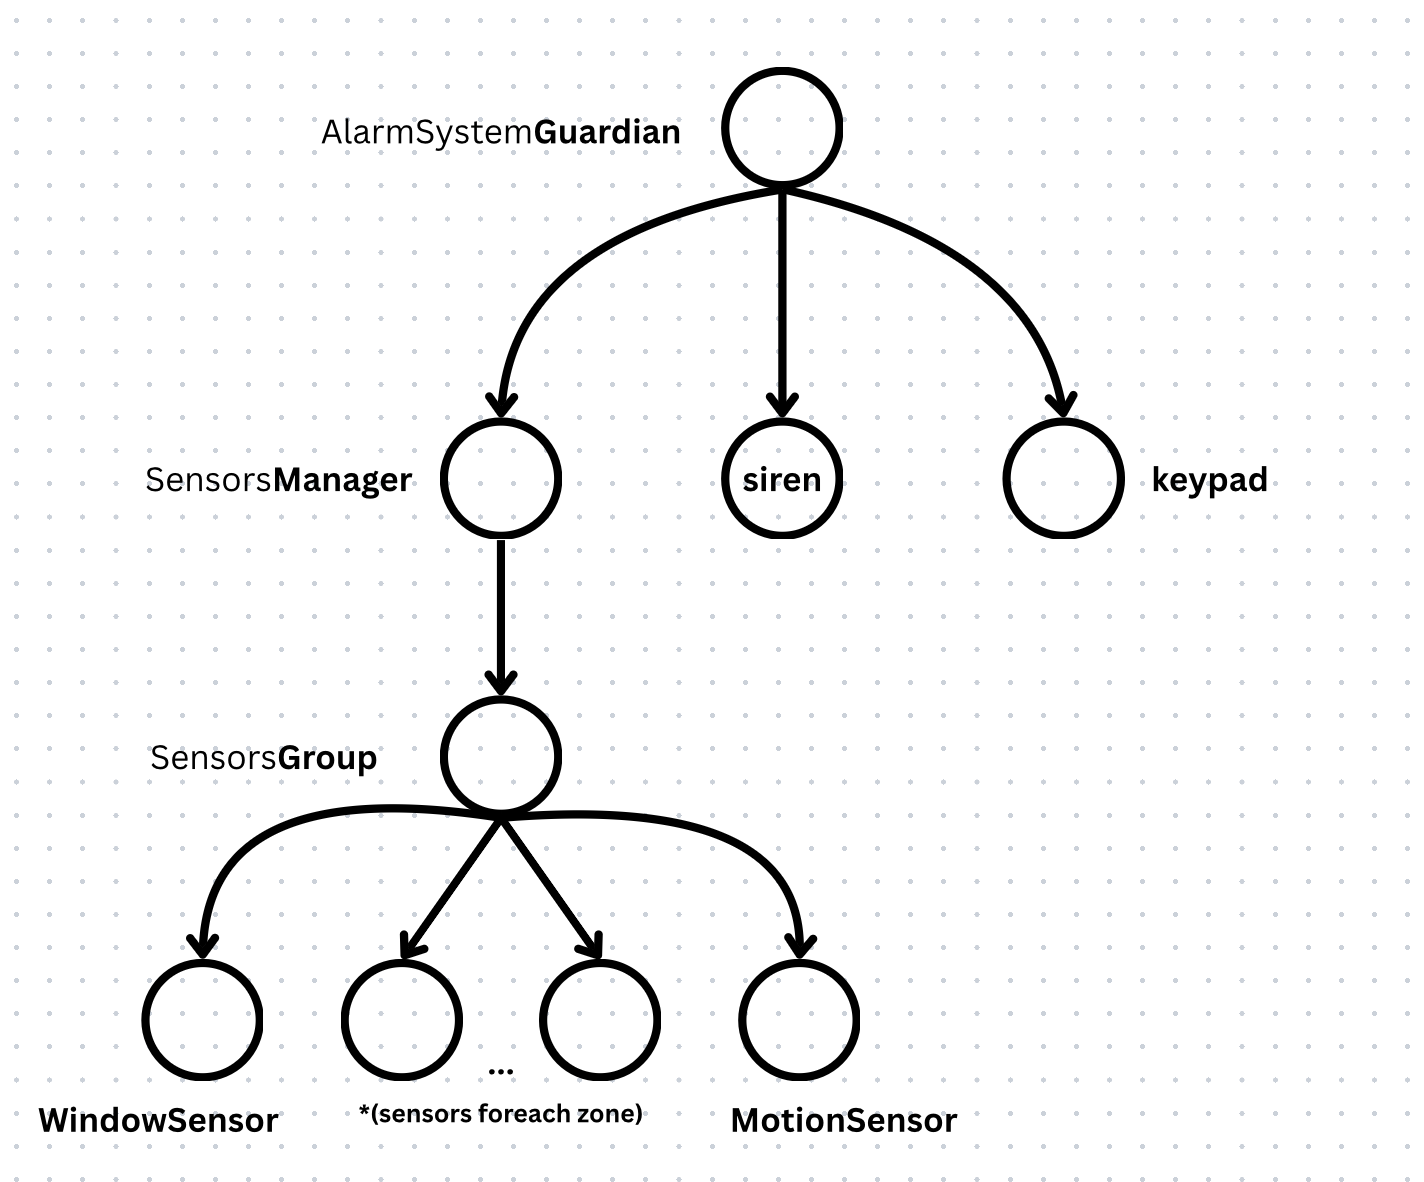
\includegraphics[width=0.8\textwidth]{figures/tree.png}
\end{center}

\begin{itemize}
    \item \textbf{KeypadActor} (keypad): Si occupa di segnalare input dell'utente.
    \item \textbf{SirenActor} (siren): Si occupa di attivare l'allarme sonoro.
    \item \textbf{SensorsManager}: Un attore intermediario che funge da router. \texttt{AlarmSystemGuardian} delega a lui la totale creazione e gestione dei sensori.
    \item \textbf{SensorsGroup}: Mantiene la suddivisione dei sensori in zone, occupandosi di propagare i comandi di armamento / disarmamento in modalità broadcast ai \textbf{SensorsActors}.
    \item \textbf{SensorsActors}: Definisce il comportamento di ciascun sensore individuale (\texttt{MotionSensor} e \texttt{WindowSensor}).
\end{itemize}

\subsubsection{Modellazione del Guardian}
Invece di utilizzare variabili di stato mutabili condivise, la macchina a stati nel \textbf{AlarmSystemGuardian} è stata implementata sfruttando il \textit{Behavior Switching} di Pekko. Ogni stato del sistema restituisce un nuovo \textbf{Behavior[Command]} che definisce esattamente quali messaggi sono accettati e come reagire in quella specifica fase, ignorando o gestendo diversamente i trigger fuori contesto.

Per i vincoli temporali, è stato utilizzato il pattern \textbf{Behaviors.withTimers}. L'attore avvia timer non bloccanti (\emph{startSingleTimer}) che, allo scadere, auto-inviano un messaggio interno (es. \texttt{ExitTimeExpired} o \texttt{EntryTimeExpired}), innescando la transizione di stato in modo puramente guidato dagli eventi.

\subsubsection{Gestione delle Zone e dei Sensori}
Il \textbf{SensorsManager} definisce con un factory pattern le regole di \texttt{spawn} dei sensori: Per ogni \textbf{Zones.Zone} vengono creati un \textbf{WindowSensor} e un \textbf{MotionSensor}, tale pattern è utilizzato per delegare al \textbf{SensorsGroup} la creazione dei sensori, per quella specifica zona, e mantenere così una chiara separazione delle responsabilità.

I sensori sono progettati in modo generico con \textbf{GenericSensor}, che definisce il comportamento comune di tutti i sensori, in questo modo è possibile creare più tipologie di sensori, che avranno lo stesso comportamento base nel sistema, ovvero l'invio del segnale di allerta (\texttt{Trigger} e \texttt{SetArmed(isArmed)}).

La logica di armamento per zona, è gestita dal Guardian, è lui che decide quali zone devono essere armate o disarmate, il sensore si occuperà di inviare il segnale di allerta, solo se il sensore è armato.

\subsubsection{Supervisione e Signal}
Per garantire la robustezza e rilevare i guasti ai sensori, è stato implementato un meccanismo di intercezione di segnali per i \textbf{SensorsActors}. Nel \texttt{SensorsGroup}, ogni sensore generato viene osservato esplicitamente tramite \texttt{context.watch(sensor)}.
Se un sensore lancia un'eccezione o viene terminato, il \textbf{SensorsGroup} intercetta il segnale \textbf{Terminated} tramite la \textbf{receiveSignal} e notifica immediatamente il Guardian con un messaggio di \texttt{SensorOffline}, permettendo al sistema di gestire il caso in base al suo stato.

Per gli attori \textbf{KeypadActor} e \textbf{SirenActor}, il Guardian applica invece una \newline \texttt{SupervisorStrategy.restart} per gestire eventuali fallimenti transitori e ripristinare il loro stato pulito.

\subsection{Conclusioni e Test}
Ho utilizzato scalatest per implementare non proprio dei test automatizzati, ma un ambiente hardcoded, rendendo intiutivi i test principali. Inoltre nel main è presente un esecuzione interattiva, che permette di inserire I/O da console per testare il sistema in modo dinamico.